\section{Trabalhos Relacionados}
\label{trabalhosrelacionados}

\begin{figure*}
	\center{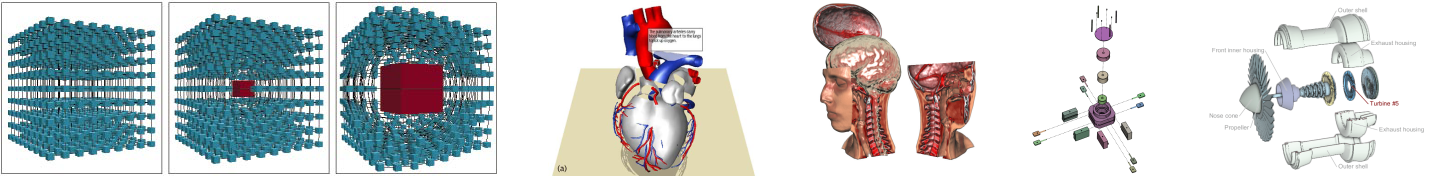
\includegraphics[width=1.0\linewidth]{img/trabalhosrelacionados.png}}
	\caption[]{\label{fig:trabalhosrelacionados} Trabalhos relacionados (\cite{857608}, \cite{1081497}, \cite{1187828}, \cite{882352}, \cite{1360700}).}
\end{figure*}

O trabalho apresentado em \cite{Viola-05-Smart} faz um levantamento de diversas t�cnicas desenvolvidas com o objetivo de facilitar a visualiza��o de modelos complexos e, por ser bastante abrangente, serve como uma base para o estudo da �rea. Em \cite{1446259}, os autores prop�e uma taxonomia para classificar essas diversas t�cnicas, apresentando os pontos positivos e negativos de cada uma.

Os trabalhos relacionados a vis�o explodida podem ser divididos em dois grupos. Uma primeira s�rie de trabalhos busca criar vistas explodidas com base em dados volum�tricos. O primeiro a explorar essa �rea foi \cite{857608}, onde os autores os autores descrevem a t�cnica \emph{visual access distortion}, que busca criar um caminho de visualiza��o sem obstru��es at� a parte de maior interesse. Os trabalhos \cite{1187828} e \cite{1081497} apresentam propostas para a visualiza��o de dados volum�tricos com vistas explodidas.

Uma outra vertente na pesquisa de vistas explodidas � baseada na explos�o de modelos 3D complexos, n�o baseados em dados volum�tricos. O trabalho \cite{882352} � uma refer�ncia inicial neste assunto e apresenta um sistema para gera��o de instru��es de montagem, mas n�o prop�e nada relacionado a vistas explodidas em espec�fico. Esse tema s� � abordado no artigo \cite{1360700}, que busca justamente expandir as instru��es de montagem e criar um sistema para a visualiza��o de vistas explodidas, dada a semelhan�a entre os dois assuntos.

Outro trabalho tamb�m relacionado a vistas explodidas � \cite{641493}, onde os autores apresentam um sistema para a gera��o autom�tica de vistas explodidas de ambientes arquitet�nicos.